\section{Anatomia alarmu}
\label{chapter:monitoring:anatomy_of_alarm}

    Alarm, z pominięciem jego biznesowego znaczenia, jest niczym więcej jak funkcją logiczną zwracającą:
    \begin{itemize}
        \item prawdę, wskazującą no to, że alarm jest obecnie aktywny, przekroczone zostały więc
        pewne wartości graniczne dla niego zdefiniowane,
        \item fałsz, alarm jest obecnie nieaktywny, a system lub komponent pracuje zgodnie z założeniami.
    \end{itemize}
    Czasami definiuje się funkcję, która zwrócić może 3 wartości. Dodatkowa możliwość sugeruje brak 
    potrzebnych danych, a alarm w takim wypadku, znajdować się może w stanie nieokreślonym. Na tym poziomie alarm
    jest podobny do neuronu w komputerowych sieciach neuronowych, a w rzeczywistości zachowuje się podobnie tak jak on.
    Jedną z czynności zalecanych przy monitorowaniu jest okresowe dostosowanie jej konfiguracji, uczenie całego
    systemu w taki sposób, aby wszelkie zgłaszane incydenty były nimi naprawdę. Fałszywy alarm, może
    przynieść więcej problemów niż korzyści. Także otrzymywanie, kilkunastu razy na dobę, powiadomień odnośnie przekroczenia 
    np. zużycia procesora może oznaczać niepoprawną konfigurację i całkowicie normalne działanie systemu.
    
    \begin{figure}[H]
        \centering
        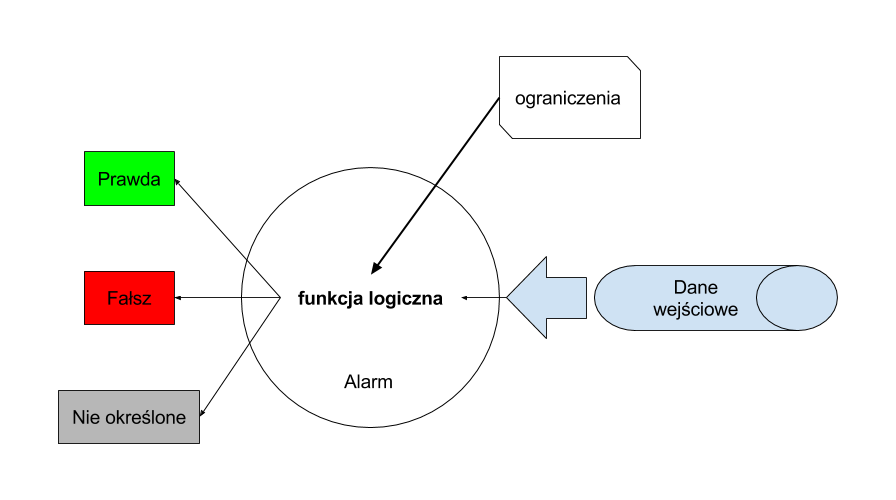
\includegraphics[width=1.0\textwidth]{images/alarm_anatomy}
        \caption[Anatomia alarmu]{Anatomia alarmu, źródło: {opracowanie własne}}
        \label{chapter:monitoring:anatomy_of_alarm:picture}
    \end{figure}
   
    \subsection{Dane wejściowe}
    Wejściem dla danej funkcji mogą być metryki, inne alarmy lub funkcje czasu. Teoretycznie jednak nie ma ustalonej
    ilości ani rodzaju możliwych wejść, a wszystko zależy od danej implementacji. Za każdym razem, kiedy 
    zmianie ulegnie stan systemu, następuje weryfikacja ograniczeń alarmu oraz reakcji na ewentualne ich
    przekroczenie. Warto w tym miejscu nadmienić, że alarmy najczęściej dodatkowo definiują również 
    konkretną liczbę przekroczeń przed aktywacją. Bez tego rozwiązania mogłoby dojść do sytuacji, w których
    alarmy przechodziłyby bardzo często ze stanu aktywnego do spoczynku, powodując generowanie dużej ilości notyfikacji. Dodatkowo alarm określa także jak wiele punktów nie aktywujących go, powinno
    nastąpić, aby przeszedł w stan nieaktywny.
    
    \subsection{Ograniczenia}
    Ograniczenia alarmu mogą być zarówno górne (<, <=) jak i dolne (>, >=). Pierwsze z nich stosowane są
    najczęściej dla sytuacji, kiedy konieczna jest wiedza o przekraczaniu przez aplikację pewnych wartości.
    Przykładem może być zwiększony czas odpowiedzi strony. Sa to najczęściej używane limity, dzięki którym
    administrator systemu jest powiadamiany o zbyt dużym zużyciu zasobowym systemów, mogących prowadzić
    do czasowego lub całkowitego jego wyłączenia. Ograniczenia dolne natomiast najczęściej
    stosowane są do mierzenia wydajności komponentów. Przykładowo, oczekuje się, że ilość wiadomości
    przepływająca przez kolejkę będzie utrzymała się na zadanym poziomie. Znając szybkość z jaką dane 
    wpływają do niej, fakt, że szybkość z jaką ją opuszczała spadła i utrzymuje się poniżej zakładanego
    limitu, może być dla administratora sygnałem wskazującym na konieczność interwencji.
    Wspomniane ograniczenia mogą być również łączone z użyciem alternatywy. Fakt aktywacji takiego
    alarmu może zostać wykorzystany w sposób ogólny do śledzenia wszelkich odchyleń od normy \cite{monitoring_and_alerting}.
    
    \subsection{Wiązania alarmów ze sobą}
    Alarmy mogą być ze sobą łączone. Ponieważ są one, z jednego punktu widzenia, funkcją
    zwracają prawdę lub fałsz, możliwe jest aby jeden alarm był jednym ze składników wejścia innego.
    W ten sposób budowane są całe hierarchie odzwierciedlające kompleksowość systemu. 
    
    \subsection{Wykluczanie}
    
        Wykluczanie odnosi się do czasowego wymuszenia na danym alarmie pozostania w stanie nieaktywnym.
        Może to zostać osiągnięte w sposób manualny lub automatyczny. W pierwszym wypadku konieczne jest,
        aby operator wznowił działanie alarmu po upływie okresu, kiedy konieczne było, aby nie
        generował on żadnych powiadomień. Wykluczania automatyczne opierają się natomiast na podstawowej własności
        alarmu - funkcji logicznej. Możliwe jest więc zdefiniowane monitora - alarmu, który wchodząc
        w stan aktywności byłby informacją dla innych alarmów, aby pozostać w stanie spoczynku. Jednocześnie
        mógłby on generować notyfikacje, jeśli byłoby to konieczne.
    
        \subsubsection{Rola funkcji czasu}
        Funkcje czasu, w przypadku wykluczeń alarmów, są szczególnie użyteczne jeśli ich intencją jest czasowe wyłączenie
        alarmu. Przykładowo w godzinach nocnych najczęściej przeprowadzane operacje sprowadzają się do zadań 
        administracyjnych, indeksacji danych lub czyszczenia systemu. Zadania tego typu mogą wymagać dużo
        zasobów systemowych, zarówno w postaci czasu procesora, jak również pamięci, przestrzeni dyskowej i sieci.
        Alarmy zdefiniowane dla tych zasobów mogłyby zostać więc aktywowane, jednak wspomniane zadania
        są planowane. Innymi słowy metryki, które podczas normalnego działania systemu, mogłoby wskazywać
        na poważny problem, dla wspomnianych operacji są zupełnie normalne.  
    
    \subsection{Łączenie}
    \label{chapter:monitoring:anatomy_of_alarm:assocation}
    
        Alarmy najczęściej odnoszą się do pojedynczej metryki, jednak jedną z możliwości, jakie alarm może
        oferować, jest łączenie metryk poprzez alarmy, na zasadach podobnych do łączenia wyrażeń
        logicznych w algebrze Bool'a. Główną zaletą agregowania alarmów jest minimalizacja powiadomień, 
        które dotyczą tego samego, a jedyną różnicą jest miejsce, czyli serwer, na którym nastąpiło
        przekroczenie wartości granicznych. 
    
        \subsubsection{Koniunkcja}
        \label{chapter:monitoring:anatomy_of_alarm:assocation:and}
        Dla tego typu asocjacji alarm przechodzi w stan aktywny tylko wtedy, jeśli wszystkie wyrażenia
        zwracają wartość logiczną równą \textbf{Prawda}. Matematycznie powyższe twierdzenie przyjmuje postać
        \mint{text}|wynik=(Alarm1 AND Alarm2 AND ... AND AlarmN)|
        Tego typu alarmy nadają się idealnie
        do monitorowania stanu klastra. Przykładowo, powiadomienie mogłoby zostać wysłane dopiero 
        wtedy, kiedy każda z maszyn będących jego częścią, przestałaby odpowiadać. Innymi słowy,
        alarm zdefiniowany dla każdego hosta wszedłby w stan aktywny. Wynika z tego, że koniunkcja
        w przypadku alarmów jest idealnym rozwiązaniem, jeśli monitoruje się stan więcej niż jednego
        komponentu, z których każdy może ulec awarii. Nie wpłynie to jednak na stan całego klastra, dopóki
        pozostałe maszyny działają.
        
        \subsubsection{Alternatywa}
        To nic innego, jak odwrotność dla koniunkcji. Matematycznie reprezentowana za pomocą wyrażenia
        \mint{text}|wynik=(Alarm1 OR Alarm2 OR ... OR AlarmN)|
        Zgodnie z logiką Bool'a wystarczy, aby jeden
        składnik wyrażenia był logiczną \textbf{Prawdą}, aby całość przyjęła taką samą wartość. \textbf{Alternatywa}
        nadaje się więc do definiowania alarmów, gdzie każda z monitorowanych encji ma krytyczne znaczenie dla działania całego systemu.
        Powołując się na przykład opisany w \ref{chapter:monitoring:anatomy_of_alarm:assocation:and}, tego typu
        alarm mógłby wejść w stan aktywny jeśli klaster komponentu A (serwer bazy danych) przestałby działać. W tym momencie pozostałe
        elementy, zarówno zgrupowane w klaster i nie, zaczęłyby zgłaszać błędy wynikające z utraconej łączności
        z bazą danych.
        
        \subsubsection{Zliczanie}
        Stanowi kompromis między \textbf{koniunkcją} a \textbf{alternatywą}. Podczas gdy pierwszy rodzaj łączenia działa
        w imię zasady - wszystko albo nic, a w przypadku drugiego, wystarczy tylko jeden argument prawdziwy, zliczanie oferuje możliwość
        zdefiniowania minimalnej liczby warunków do spełniania, aby alarm przeszedł w stan aktywny.
        Matematyczny zapis wygląda następująco:
        \mint{text}|wynik=[(Alarm1 + Alarm2 + ... + AlarmN) = K]|
        Innymi słowy operator może zdefiniować alarm następującej postaci: jeśli na 4 z 5 serwerów zużycie przestrzeni dyskowej
        wzrośnie powyżej 80 procent, należy automatycznie uruchomić procedurę archiwizacji danych \cite{monitoring_and_alerting}. 